\section{Results}
\label{sec:results}

\subsection{Test 1: four new panels}
\label{sec:v2test}
Table~\ref{tab:v2test} reports the first final test (371{,}520 learner jobs). All three steps pass. Against the robust head on the 228 pooled external MDPs, \OEH{} improves IBS by $0.0171$ (LB $+0.0107$) and LL by $0.0597$ ($+0.0344$). Inside the generator it is non-inferior to OEH-F (LB $+0.0003$ and $+0.0045$ on $1.02\cdot\text{OEH-F}-\OEH{}$; the forecasts nearly coincide, since the median $d$ is 1.1), and outside it beats OEH-F by $0.0047$ ($+0.0028$) and $0.0662$ ($+0.0398$). All 24 step-3 bounds are positive. Relative to B2 matched, \OEH{} lowers IBS and LL by 15.7\% and 8.3\% inside the generator and by 37.7\% and 23.4\% outside, with per-panel intervals excluding zero everywhere. The margin over the robust head, however, comes from forest management ($+0.070$ IBS, $+0.23$ LL); on Colosseum it is not individually significant ($+0.0074$ $[-0.0055,0.0204]$), on SPIBB-2 the methods tie, and without forest the pooled gain is $+0.0030$ $[-0.0022,0.0082]$. The only learner cells where \OEH{} is significantly worse than OEH-F are the all-censored BC and IQL rows of SPIBB-2, by at most 0.003 nat, within Proposition~\ref{prop:gate}.

\begin{table*}[t]
\centering
\caption{Test 1 (IBS / LL, MDP-averaged; lower is better; best in bold). Gate: step 1 vs the robust head on the pooled external MDPs, LB $+.0107$ / $+.0344$; step 2 non-inferiority to OEH-F inside (LB $+.0003$ / $+.0045$) and superiority outside (LB $+.0028$ / $+.0398$); step 3 all 24 contrasts positive.}
\label{tab:v2test}
\footnotesize
\setlength{\tabcolsep}{4pt}
\begin{tabular}{@{}lccccc@{}}
\toprule
Method & Internal (168) & Colosseum 2029 (72) & SPIBB-2 (108) & Forest (48) & Pooled external (228)\\
\midrule
\OEH{} & .0476 / \textbf{.562} & \textbf{.1080} / \textbf{.833} & .0189 / .358 & \textbf{.1097} / \textbf{.790} & \textbf{.0662} / \textbf{.599}\\
OEH-F (no gate) & \textbf{.0475} / .563 & .1153 / .951 & \textbf{.0188} / \textbf{.352} & .1216 / .941 & .0709 / .665\\
Robust head (B2 + D) & .0497 / .579 & .1154 / .873 & .0190 / .354 & .1794 / 1.022 & .0832 / .659\\
B2 + LCE & .0544 / .597 & .1396 / .995 & .0249 / .400 & .1299 / .865 & .0832 / .686\\
B2 matched & .0565 / .613 & .1407 / .989 & .0252 / .420 & .2370 / 1.285 & .1063 / .782\\
XGBoost-CF/18 & .0596 / 1.122 & .1436 / 1.256 & .0277 / .457 & .2535 / 1.447 & .1118 / .918\\
\bottomrule
\end{tabular}
\end{table*}

\subsection{Tests 2 and 3: four new sources}
\label{sec:fifth}
\textbf{Test 2} registered only the contrast with the robust head, on 72 MDPs from FrozenLake (slippery) and the gambler's problem. It is \textbf{NO-GO}: \OEH{} changes IBS by $-0.0017$ (LB $-0.0067$) and LL by $+0.0117$ ($-0.0196$). On FrozenLake every requirement is censored; \OEH{} recognizes this far better than the robust head ($+0.0065$ IBS, $+0.072$ LL), but the learner's own pilot learning curve (LCE) is better still. On the gambler's problem the robust head is better, mainly for BC. Descriptively, \OEH{} again beats OEH-F ($+0.0009$ IBS, $+0.020$ LL, intervals excluding zero) and B2 in LL ($+0.058$ $[0.031,0.086]$) (Table~\ref{tab:fifth}).

\begin{table}[t]
\centering
\caption{Test 2 (IBS / LL). Registered contrast \OEH{} vs robust head: NO-GO. All FrozenLake requirements are censored.}
\label{tab:fifth}
\footnotesize
\setlength{\tabcolsep}{3pt}
\begin{tabular}{@{}lccc@{}}
\toprule
Method & FrozenLake (36) & Gambler (36) & Pooled (72)\\
\midrule
\OEH{} & .0040 / .082 & .0931 / .752 & .0486 / \textbf{.417}\\
OEH-F (no gate) & .0038 / .079 & .0951 / .795 & .0495 / .437\\
Robust head (B2 + D) & .0105 / .154 & .0831 / \textbf{.703} & \textbf{.0468} / .428\\
B2 matched & .0122 / .153 & .0958 / .797 & .0540 / .475\\
LCE raw & \textbf{.0007} / \textbf{.025} & .1132 / 1.174 & .0569 / .599\\
$k$-NN analog on B2 & .0176 / .243 & \textbf{.0795} / .728 & .0486 / .485\\
\bottomrule
\end{tabular}
\end{table}

\textbf{Test 3} asks whether the advantage lies in the budgets the pilot cannot reach and survives the strongest pilot-extrapolation baseline, on 96 MDP Playground and 96 labmaze MDPs (230{,}400 learner jobs). Both registered families pass (Table~\ref{tab:panel6}): against B2 + prefix/FQE, \OEH{} improves $\mathrm{IBS}_\ge$ by $0.0315$ (LB $+0.0247$) and $\mathrm{LL}_{\rm ext}$ by $0.1034$ ($+0.0808$), that is, by 25.6\% and 17.9\%; against B2 by 43.8\% and 32.8\% (LB $+0.0616$, $+0.2025$). Under the registered decision rule \OEH{} also lowers regret, by 2.61 budget units against B2 + prefix/FQE (LB 1.29) and by 7.91 against B2 (LB 6.13); F3 is an estimate without a verdict. The labels are not degenerate: 22--84\% of rows are censored, depending on learner and family.

Three descriptive results go against parts of the design. (i) \emph{The gate hurt}: OEH-F beats \OEH{} by 3.3\% in IBS and 3.6\% in LL (intervals excluding zero). Almost all of this is on MDP Playground, where 71\% of groups lie at $d\ge3$ and the robust head's finite law transferred worse than the full head's; on labmaze the two tie. (ii) \OEH{} beats the robust head by 14.8\% IBS, significantly only on labmaze, so across the three tests the comparison with the robust head is panel-dependent in both directions. (iii) On MDP Playground, whose rewards are dense, the raw pilot learning curve has the lowest IBS (OEH is 32.7\% worse) but a worse log loss and no advantage on the extrapolation endpoint.

\begin{table}[t]
\centering
\caption{Test 3: full scores by family (IBS / LL) and the registered extrapolation endpoint, pooled over 192 MDPs ($\mathrm{IBS}_\ge$ / $\mathrm{LL}_{\rm ext}$). Gates F1 (vs B2 + prefix/FQE) and F2 (vs B2): GO.}
\label{tab:panel6}
\footnotesize
\setlength{\tabcolsep}{2.2pt}
\resizebox{\columnwidth}{!}{%
\begin{tabular}{@{}lccc@{}}
\toprule
Method & MDP Playground & labmaze & Pooled, extrapolation\\
\midrule
\OEH{} & .1176 / 1.211 & \textbf{.0767} / .867 & .0915 / .475\\
OEH-F (no gate) & .1104 / \textbf{1.151} & .0777 / \textbf{.855} & \textbf{.0858} / \textbf{.451}\\
Robust head (B2 + D) & .1226 / 1.239 & .1053 / 1.005 & .1147 / .556\\
B2 + prefix/FQE & .1347 / 1.209 & .1024 / .969 & .1229 / .579\\
B2 + LCE & .1350 / 1.277 & .0962 / .956 & .1175 / .549\\
LCE raw & \textbf{.0886} / 1.234 & .1294 / 1.434 & .1289 / .767\\
TabPFN v2 on B2 & .1563 / 1.329 & .1269 / 1.072 & .1463 / .640\\
B2 matched & .1740 / 1.501 & .1326 / 1.092 & .1629 / .708\\
\bottomrule
\end{tabular}}
\end{table}

\begin{figure}[t]
\centering
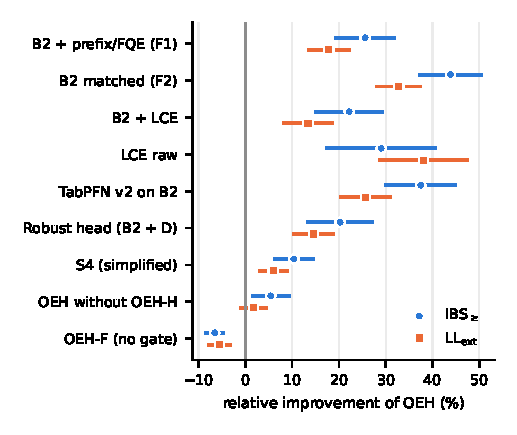
\includegraphics[width=\columnwidth]{figures/fig_panel6.pdf}
\caption{Test 3: relative improvement of \OEH{} over each comparator on the registered extrapolation endpoint, pooled over 192 MDPs; bars are 95\% MDP-cluster intervals of the absolute difference divided by the comparator's mean. The first two rows are the registered gates; the others are descriptive.}
\label{fig:panel6}
\end{figure}

\subsection{Is the gain retrospective?}
\label{sec:retro}
A forecaster could score well on $x1$--$x5$ by retrodicting what the pilot shows. On the opened panels, rescored post hoc on Eq.~\eqref{eq:ext}, the gain of \OEH{} over B2 on the extrapolation endpoint is at least as large as on the full endpoint in every scope (Test 1 external: 39.8\% $\mathrm{IBS}_\ge$, 26.2\% $\mathrm{LL}_{\rm ext}$; internal: 17.4\%, 11.2\%). The prefix/FQE baseline in its raw form is not competitive (LL 1.7--2.3 on 9 of 11 panels), but calibrated by the matched head it beats B2 by 18.4\% IBS on Test 1's external panels; \OEH{} still beats it there by 23.7\% IBS and 13.0\% LL. Test 3 then confirmed this ordering prospectively. Running the learner on the pilot is informative, but it is not enough.

\subsection{Where the gain comes from}
\label{sec:mechanism}
Fig.~\ref{fig:distance} pools the rows of Test 1 by shift distance. Near the training data ($d\le1.5$) the three predictors gain alike over B2; beyond $d_0=3$ the gate's combination beats both of its heads (at $d>4$: 0.32 nat for \OEH{}, 0.23 for the robust head, 0.11 for OEH-F), because it pairs the full head's censored probability with a finite law that transferred better there. Test 3 shows that this is not guaranteed. The distance sees only B2 statistics, so a change of logging behavior is invisible: SPIBB lies at $d\approx1.9$, and on the two SPIBB panels no method wins clearly. In the Murphy decomposition, \OEH{} and OEH-F gain mainly by \emph{resolution} outside the generator (Test 3: 0.12--0.13 against 0.06 for B2), not uniformly by calibration.

\begin{figure}[t]
\centering
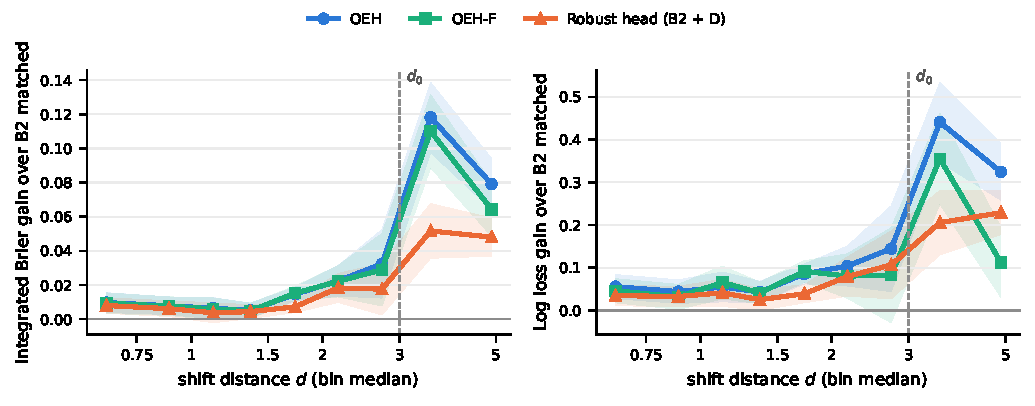
\includegraphics[width=\columnwidth]{figures/fig_gain_by_distance.pdf}
\caption{Gain over B2 by shift distance $d$ on Test 1 (rows pooled in nine bins; shaded: 95\% intervals; descriptive). The dashed line marks $d_0$.}
\label{fig:distance}
\end{figure}

\textbf{Features or learner?} TabPFN v2 on the 18 B2 statistics \emph{ties} \OEH{} inside the generator (\OEH{} is 1.9\% better in IBS and 0.7\% worse in LL, both intervals including zero), so most of the in-generator gain over B2 matched is reproduced by a stronger tabular learner on generic statistics. Outside the generator TabPFN only ties B2, and \OEH{} beats it by 37.4\% IBS and 19.5\% LL on Test 1 and by 31.4\% and 13.5\% on Test 3, where it was sealed before the labels. The value of the \OEH{} features lies in transfer.

\textbf{Components.} Inside the generator the information blocks are redundant: in a same-head leave-block-out on the opened cohort 7, removing any single block costs at most 1.4\% IBS. Outside it, rebuilding \OEH{} without OEH-H worsens Test 1's external IBS by $0.0028$ $[0.0012,0.0044]$ and Test 3's by $0.0048$ $[0.0023,0.0074]$, and without the direct posterior simulation worsens Test 1's external LL by $0.022$ $[0.011,0.033]$. Four simplified single-head candidates, specified with an acceptance rule before they were run, all failed it on 11 opened panels (the closest, S4, was 3.3\% worse outside and 8.0\% worse in IBS on Test 3). A nested leave-one-panel-out rerun of the whole gate selection puts its optimism at about one percentage point ($-5.6\%$ held-out vs $-6.6\%$ for one fit on all five panels, relative to OEH-F). These analyses are descriptive; no component claim is confirmatory.

\textbf{Label definition.} Rescoring the sealed forecasts on labels redefined with $\tau\in\{0.90,0.95,0.99\}$ and 7--9 of 10 seeds (reproducing all 11{,}988 official labels at $0.95$, 8/10), \OEH{} beats B2 outside the generator in all nine cells, but inside it is significantly \emph{worse} at $\tau=0.99$ (IBS $-8$ to $-10\%$): a forecaster fitted sharply for one target is penalized more when the target moves. On Test 3 the registered $\tau=0.99$ variant keeps the external ordering (\OEH{} .0964 / .989, B2 + prefix/FQE .1254 / 1.102, B2 .1554 / 1.233).

\subsection{Development evidence and negative results}
\label{sec:development}
Before the gate existed, OEH-F was tested on a sealed cohort of 84 generator MDPs: it lowered IBS by 15.97\% and LL by 10.22\% relative to B2, and all 22 registered contrasts, including two privileged ones, had positive simultaneous bounds. The gain was clear for CFQI and IQL, uncertain for BC (90.7\% censored) and absent for bottleneck MDPs. Table~\ref{tab:replication} lists the later development panels. On Colosseum, 77--98\% of the IBS gain came from censored rows and OEH-F's finite-budget law was worse than B2's: replacing it lowered OEH-F's LL from 0.890 to 0.856, which motivated the gate. Three earlier formulations failed their own sealed tests. On published BRIDGE MDPs~\cite{laidlaw2024stochastic}, with our pilots and labels, OEH-F was learner-dependent (better for CFQI, worse for IQL on Atari), and on the FourRooms offline log~\cite{farama_minari_fourrooms} the Dirichlet transition component lost to maximum likelihood.

\begin{table}[t]
\centering
\caption{Development panels of OEH-F (IBS / LL). LB: simultaneous lower bound of the improvement over B2.}
\label{tab:replication}
\footnotesize
\setlength{\tabcolsep}{2.2pt}
\resizebox{\columnwidth}{!}{%
\begin{tabular}{@{}lrcccc@{}}
\toprule
Panel & MDPs & OEH-F & B2 & LB vs B2 & vs robust head\\
\midrule
Cohort 7 (sealed) & 84 & .0460 / .563 & .0547 / .627 & $+.0027$ / $+.030$ & ---\\
Cohort 8 & 168 & .0466 / .548 & .0566 / .614 & $+.0066$ / $+.047$ & GO\\
Colosseum 2027 & 72 & .1010 / .890 & .1342 / .982 & $+.0151$ / $+.0003$ & NO-GO\\
Colosseum 2028 & 72 & .1050 / .895 & .1436 / 1.000 & $+.0176$ / $+.0060$ & NO-GO\\
SPIBB & 108 & .0192 / .366 & .0209 / .387 & $-.0005$ / $-.0060$ & ---\\
\bottomrule
\end{tabular}}
\end{table}

\subsection{Selection, cost and decision value}
\label{sec:cost}
\textbf{Selection.} A selector frozen before cohort 7's outcomes, using CFQI's pilot features, its OEH-F probabilities and the MDP-family label, chose among seven learners at $x10$. Against fixed CFQI it raised seed success by 6.67 points (LB $+4.26$) and normalized return by 0.0187 ($+0.0103$); against an earlier internal router the bounds crossed zero. \textbf{Cost.} Posterior simulation dominates \OEH{}'s cost (67\% of the pilot-input time on Test 1's internal panel; median 10.7\,s per MDP--behavior pair), grows quickly with $SA$ and exceeded our dense-model cap on most BRIDGE tasks; the gate adds no measurable cost. \textbf{Decision value.} Under the registered rule (collect the smallest budget whose forecast success probability reaches $q=0.8$, penalty $\kappa=100$), regret on Test 1 is 13.1 for \OEH{}, 15.1 for the robust head and 16.5 for B2 inside, and 20.0, 28.1 and 35.8 on forest; \OEH{} and OEH-F differ by at most 1.1 units on every panel. Theorem~\ref{thm:regret} and its variants hold on all four Test-1 panels but are loose (plug-in regret 4--36 units against bounds of 24--101). These figures exclude the cost of the pilot and of \OEH{}, so we make no claim of data or compute savings.

\textbf{Limitations.} All MDPs are tabular with $SA\le256$ and exact evaluation, and the label depends on a 0.95 threshold, ten seeds, an 8/10 sustained rule and a six-point grid. 71\% of meta-training rows are censored, and 91--98\% of censored rows in Test 1 still fail at $x200$. The posterior smooths the behavior and assigns zero reward to unobserved keys, which can mislead BC forecasts. The shift distance does not detect behavior shift, and adding behavior families to meta-training did not help. Inside the generator, a strong generic tabular learner matches \OEH{}.
